\section{Results}

The entire project can be subdivided into three categories.

\subsection{Transmitter}
In the transmitter section, three ultrasonic transmitters and a microcontroller AtMega8 is used to transmit a $40kHz$ in three directions. Similarly, simultaneously, three IRLED transmits $38kHz$ infrared signal in respective direction.


\subsection{Receiver}
In the receiver section, there are three receivers located at three direction. Each receiver comprise of an ultrasonic receiver, a TSOP, a three op-amp instrumentation amplifier, tone decoder and a microcontroller. Ultrasonic receiver receives the $40kHz$ ultrasonic signal while the TSOP receives the $38kHz$ infrared signal. 

Now the received ultrasonic signal is fed to the instrumentation amplifier. The outputs of instrumentation amplifier at different distances from the transmitter is shown in table \ref{tab:OpampOutput}
\begin{table}[htpb]
	\centering
	\caption{Output of instrumentation amplifier at different distances}
	\label{tab:OpampOutput}
	\begin{tabular}{|c|c|c|}
	\hline 
	Distance(cm) & Input(mV) & Output(mV) \\ 
	\hline 
	10 & 460 & 11100 \\ 
	\hline 
	20 & 115 & 2785 \\ 
	\hline 
	30 & 51 & 1238 \\ 
	\hline 
	40 & 28 & 690 \\ 
	\hline 
	50 & 18 & 440 \\ 
	\hline 
	60 & 13 & 305 \\ 
	\hline 
	70 & 9.5 & 227 \\ 
	\hline 
	80 & 7.2 & 170 \\ 
	\hline 
	\end{tabular} 
\end{table}

A graph of signal strength vs. distance was plotted and the observed graph is shown in Figure \ref{fig:Attenuation}
\begin{figure}[htpb]
	\centering
	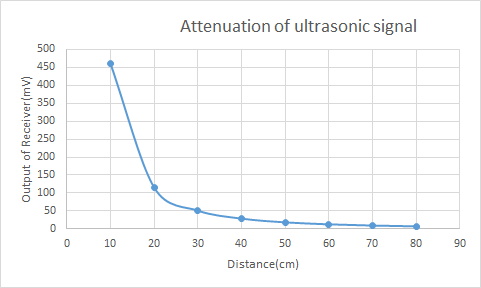
\includegraphics[scale=1]{Images/AttenuationGraph.png}
	\caption{Attenuation of signal}
	\label{fig:Attenuation}
\end{figure}

The output obtained from the instrumentation amplifier was plotted against the input at instrumentation. The observed graph is shown in Figure.\ref{fig:InputOutputGraph}
\begin{figure}[htpb]
	\centering
	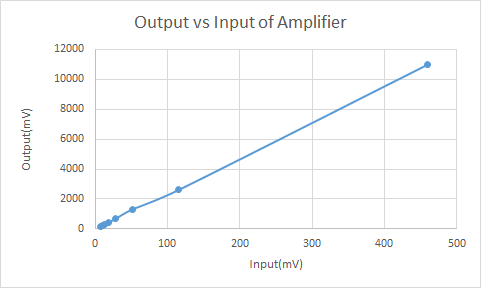
\includegraphics[scale=1]{Images/OutputvsInput.png}
	\caption{Output vs Input graph}
	\label{fig:InputOutputGraph}
\end{figure}

\subsection{Graphical User Interface}
After sending the distance information between all the ultrasonic transmitters and receivers to PC via \gls{usb} cable, the location of transmitter is determined using trilateration. Now the location of the transmitter is displayed in a \gls{gui}. One instance of locating the path of transmitter in PC is shown in Figure.\ref{fig:LiveView}
\begin{figure}[htpb]
	\centering
	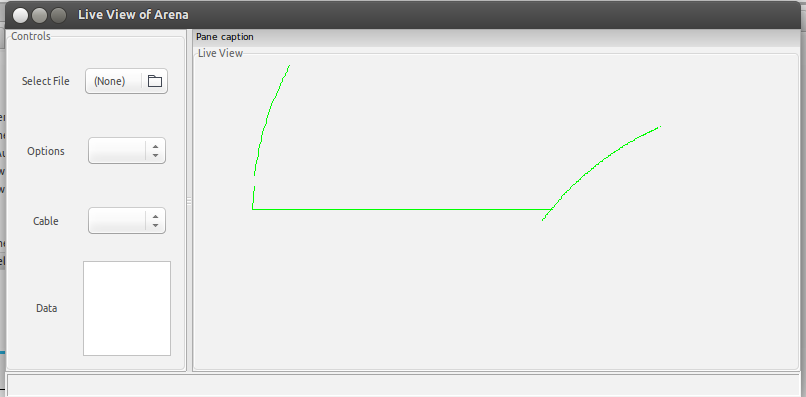
\includegraphics[scale=0.45]{Images/LiveView.png}
	\caption{Real Time View of Moving Transmitter}
	\label{fig:LiveView}
\end{figure}
